Supposons être en possession de $L$ et de $\mathcal{F}(L)$. Nous décrivons ici comment implémenter la comparaison de \fl avec $L$ selon les critères énoncés dans la section \ref{ss:fixe}.


L'algorithme de comparaison \ref{alg:comp} suppose l'existence d'opérations de base. Dans le cadre d'une implémentation, celles-ci doivent également être disponibles.

Soient deux ADF $A$ et $B$ ainsi que les langages qui sont représentés par ceux-ci, respectivement $L_A=L(A)$ et $L_B=L(B)$.
Voici une liste des opérations nécéssaires.

\begin{itemize}
    \item La conjonction : $L_A\bigcap L_B$
        \begin{figure}[H]
            \center
            \colorlet{circle edge}{black}
            \colorlet{circle area}{blue!20}
            \tikzset{
                filled/.style={fill=circle area, draw=circle edge},
                outline/.style={draw=circle edge},
                whitened/.style={fill=white, draw=circle edge}}
            \def\circleA{(0,0) circle (1cm) node {$L_A$}}
            \def\circleB{(1.5,0) circle (1cm) node {$L_B$}}
          \vspace{0.6cm}
          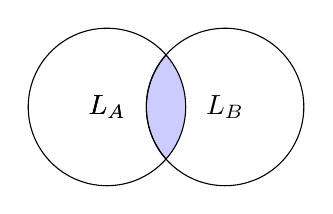
\begin{tikzpicture}
            \begin{scope}
                \clip \circleA;
                \fill[filled] \circleB;
            \end{scope}
            \draw[outline] \circleA;
            \draw[outline] \circleB;
          \end{tikzpicture}
          \caption{$L_A\bigcap L_B$ en bleu}
        \end{figure}

    \item L'équivalence : $L_A$ est-il égal à $L_B$ ?
    \item La disjonction : $L_A\bigcup L_B$
        \begin{figure}[H]
            \center
            \colorlet{circle edge}{black}
            \colorlet{circle area}{blue!20}
            \colorlet{circle darker}{blue!40}
            \tikzset{filled/.style={fill=circle area, draw=circle edge},
            outline/.style={draw=circle edge}}
            \def\circleA{(0,0) circle (1cm) node {$L_A$}}
            \def\circleB{(1.5,0) circle (1cm) node {$L_B$}}
          \vspace{0.6cm}
          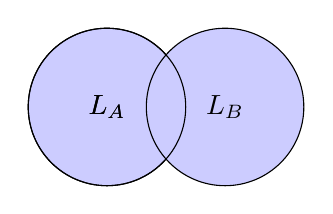
\begin{tikzpicture}
            \draw[filled]\circleA;
            \draw[filled]\circleB;
            \draw[outline]\circleA;
          \end{tikzpicture}
          \caption{$L_A\bigcup L_B$ en bleu}
        \end{figure}

    \item La disjonction exclusive ($(A\bigcup B)\backslash(A\bigcap B)$, notée $A\xor B$)
        \begin{figure}[H]
            \center
            \colorlet{circle edge}{black}
            \colorlet{circle area}{blue!20}
            \colorlet{circle darker}{blue!40}
            \tikzset{filled/.style={fill=circle area, draw=circle edge},
            outline/.style={draw=circle edge},
            whitened/.style={fill=white, draw=circle edge}}
            \def\circleA{(0,0) circle (1cm) node {$L_A$}}
            \def\circleB{(1.5,0) circle (1cm) node {$L_B$}}
          \vspace{0.6cm}
          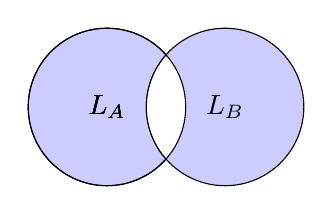
\begin{tikzpicture}
            \draw[filled] \circleA;
            \draw[filled] \circleB;
            \begin{scope}
                \clip \circleA;
                \fill[whitened] \circleB;
            \end{scope}
            \draw[outline] \circleA;
          \end{tikzpicture}
          \caption{$L_A\xor L_B$ en bleu}
        \end{figure}
    \item La différence avec le vide : $L_A=\emptyset ?$
    \item La sélection d'un mot : $w\in L_A$
\end{itemize}

La comparaison de $\mathcal{F}(L)$ avec $L$ est plus complexe qu'une simple équivalence car le contre-exemple à retourner dépend de l'automate à files $F$. En effet, le contre-exemple recherché n'est pas un contre-exemple à l'égalité $L=\mathcal{F}(L)$ mais à l'égalité $L=AL(F)$. (Voir section \ref{ss:fixe})

\begin{algo}[Comparaison]
  \begin{algorithmic}[1]
    \REQUIRE Un langage de traces annotées $L$ pour un automate à files $F$, $\mathcal{F}(L)$
    \ENSURE L'égalité entre $L$ et $\mathcal{F}(L)$ ou un contre-exemple $\gamma\in\Phi^*$ à l'égalité $L=AL(F)$
    \IF {$L=\mathcal{F}(L)$}
        \RETURN $L$ est un point fixe de $\mathcal{F}$.
    \ELSE
        \STATE $X= L\xor\mathcal{F}(L)$ \COMMENT{$X$ est non-vide car $L\neq\mathcal{F}(L)$}
        \STATE Prenons $\gamma\in X$
        \IF {$\gamma \in L$}
            \RETURN $\gamma$
        \ELSE
            \IF {$\gamma$ est une annotation valide}
                \RETURN $\gamma$
            \ELSE
                \RETURN reverseFL($\mathcal{F}(L)$, $F$, $\gamma$)
            \ENDIF
        \ENDIF
    \ENDIF
  \end{algorithmic}\label{alg:comp}
\end{algo}


A l'exception du mot $t_{q_0}$, $\mathcal{F}(L)$ contient des mots $\gamma$ tels que $\exists \gamma'\in L \exists \theta\in\Theta, \gamma=Post(\gamma',\theta)$.

Sous l'hypothèse que $\gamma$ n'est pas $t_{q_0}$, ce qui en ferait une annotation valide, rendant inutile l'appel à reverseFL, reverseFL trouve ce $\gamma'$ et $\theta$.

\begin{algo}[reverseFL]
    \begin{algorithmic}[1]
        \REQUIRE
        \begin{itemize}
            \item Un langage obtenu par la fonction $\mathcal{F}$ : $\mathcal{F}(L)$
            \item L'automate à files concerné par $L$  : $F$
            \item Une trace annotée $\gamma\in\Phi^*$
        \end{itemize}
        \ENSURE une trace annotée $\gamma'\in L$ tel que $\exists \theta, \gamma=Post(\gamma',\theta)$ s'il existe

        \IF{$\gamma$ est une trace correctement annotée}
          \STATE $\gamma' t_q \leftarrow \gamma$ avec $\gamma'\in\Phi^*,t_q\in T_Q$

          \IF {$\exists \theta_\tau$ tel que $dest(\theta_\tau)=t_q$ et l'action de $\theta_\tau$ est $\tau$}
            \IF{$\gamma'=\epsilon$ ou $dest(\gamma')=source(\theta_\tau)$}
              \RETURN $\gamma'.source(\theta_\tau)$
            \ENDIF
          \ENDIF

          \IF {$\gamma'=\gamma''.\phi$ avec $\gamma''\in\Phi^*$ et $\phi \in \Phi$}
            \IF {$\phi\in\Theta$ et $dest(\phi)=q$}
              \RETURN $\gamma''.t_{source(\phi)}$
            \ENDIF

            \FORALL {symbole $\bt\in \gamma''.\phi$ de droite à gauche tels que $\bt\in$\barTheta}
              \STATE $u_1.\bt.u_2.t_q \leftarrow \gamma$ avec $u_1,u_2 \in \Phi^*$
              \STATE $(r, c!m, s)\leftarrow\delta(\theta)$
              \FORALL {symbole $\theta_r\in\Theta$}
                \IF{ $\delta(\theta_r)=(p, c?m, q)$ avec le $q$ de $t_q$}
                  \RETURN $u_1.\theta.u_2.t_p$
                \ENDIF
              \ENDFOR
            \ENDFOR
          \ENDIF
        \ENDIF
    \end{algorithmic}
\end{algo}


\subsection{Exemple d'application de reverseFL}

Soit l'automate à files $F$ dans la figure \ref{fig:fifo1}. Supposons être en possession d'un ADF $A$ tel que $L(A)=AL(F)$.
Comme $AL(F)=\mathcal{F}(AL(F))$, reverseFL peut être employé avec $A$.
Soit la trace annotée $\gamma=\bt_2\bt_5\bt_5\bt_1\theta_4 t_{q_0} \in AL(F)$.

Voici le déroulement de $reverseFL(A,F,\gamma)$.

\begin{enumerate}
  \item $\gamma$ finit par $\theta_4\in\Theta$ mais $dest(\theta_4)\neq q_0$
  \item $\bt_0\in$\barTheta pour lequel il existe $\theta_3$ avec $\delta(\theta_3)=(q_1,a?0,q_3)$. $q_3\neq q_0$
  \item $\bt_4\in$\barTheta pour lequel il existe $\theta_7$ avec $\delta(\theta_7)=(q_3,b?0,q_0)$. $q_0$ est correct. L'algorithme retourne $\gamma'=(\bt_2\bt_5).\theta_5.(\bt_1).t_{q_3}$
\end{enumerate}

Le résultat peut être vérifié simplement : $Post(\gamma',\theta_7)=\gamma$.
